% Chapter Template

\chapter{Pile Up Studies} % Main chapter title

\label{Chapter 8} % Change X to a consecutive number; for referencing this chapter elsewhere, use \ref{ChapterX}

\lhead{Chapter 78 \emph{PU Studies}} % Change X to a consecutive number; this is for the header on each page - perhaps a shortened title

%----------------------------------------------------------------------------------------
%	SECTION 1
%----------------------------------------------------------------------------------------

\section{Jet}
\subsection{Efficiencies}
In order to test the jet finding algorithm the first study that must be undertaken is into the matching efficiency of the L1 jets to the generator level quantities for a ttbar(PU 40, $\tau_b=50ns$) MC sample. The gen jets are made by running the anti-kt 4 algorithm **REF** on the generator level quantities. The gen jet is said to be matched if within ${\Delta R}^2<33$ of a L1 jet (the greatest extent of the L1 jet). The matching efficiency for alljets and the 4 jet is shown in figure \ref{match}. It can be seen that the efficiency after PUS/seed drops at low $p_T$, however, for the trigger such jets are mainly relevant for $H_T$ which is shown to perform well. Inefficiencies at high $p_T$ are caused by the 'chain veto', however, the jet algorithm guarantees there is always a comparable or higher jet in the event in such cases. The performance compared to GCT is seen to be greatly improved.  
\begin{figure}
\hfill
\subfigure[All jets\label{fig:label:alljet}]{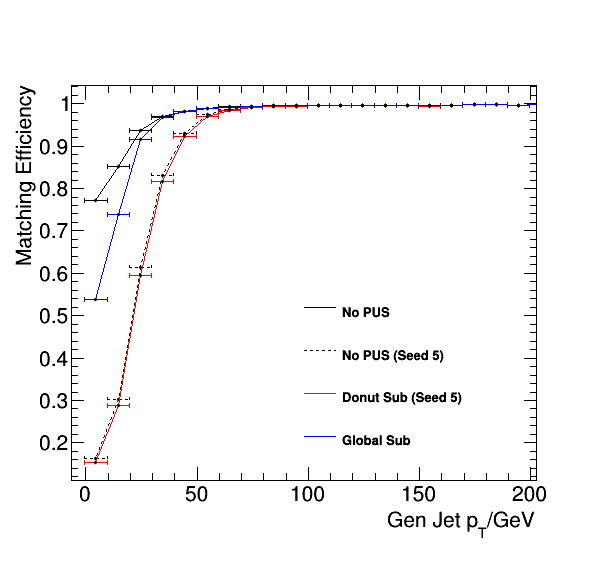
\includegraphics[width=7cm]{Figures/alljet}}
\hfill
\subfigure[4th jet\label{fig:label:jet4}]{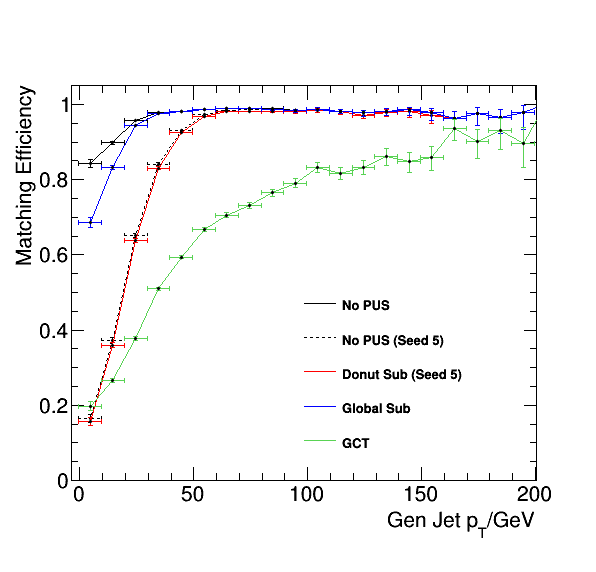
\includegraphics[width=7cm]{Figures/jet4}}
\hfill
\caption{Matching efficiencies for jets showing effect of seed and PUS at low energies. In \ref{fig:label:jet4} a comparison with the GCT is shown.}
\label{match}
\end{figure}
\subsection{Calibration}
The energy of the L1 jets must be calibrated using generator level quantities. The scheme for calibration is outlined in \cite{l1jet_calibration}. Essentially, using a QCD PU 40, 50ns sample, the resolution (defined as $p^{L1}_{T}/p^{gen}_{T}$) and $p^{L1}_{T}$ are plotted against $p^{gen}_{T}$ and fitted. The fits are then plotted against each other giving calibration factors as a function of $p^{L1}_{T}$. The calibration is carried out in bins of $\eta$ to account for the difference in performance of the detector. Where the matching efficiency is low it is not possible to fit and so the calibration has a lower bound on $p_T$. This was found to occur at $20GeV$. The calibration factors change depending on the PUS regime.    
\begin{figure}
\hfill
\subfigure[All jets\label{fig:label:alljet}]{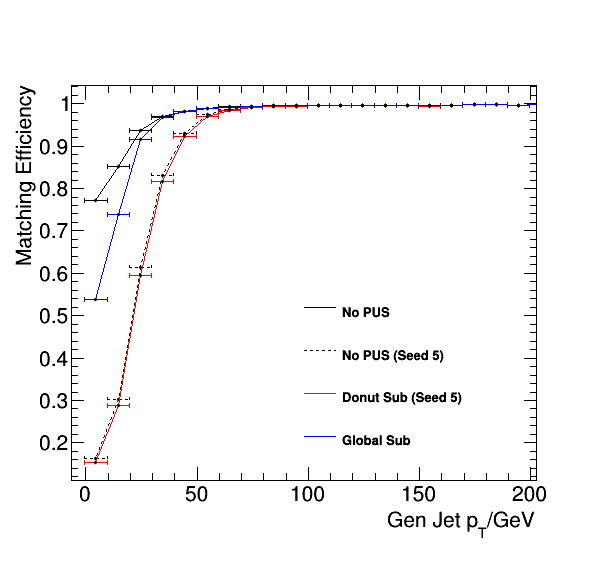
\includegraphics[width=7cm]{Figures/alljet}}
\hfill
\subfigure[4th jet\label{fig:label:jet4}]{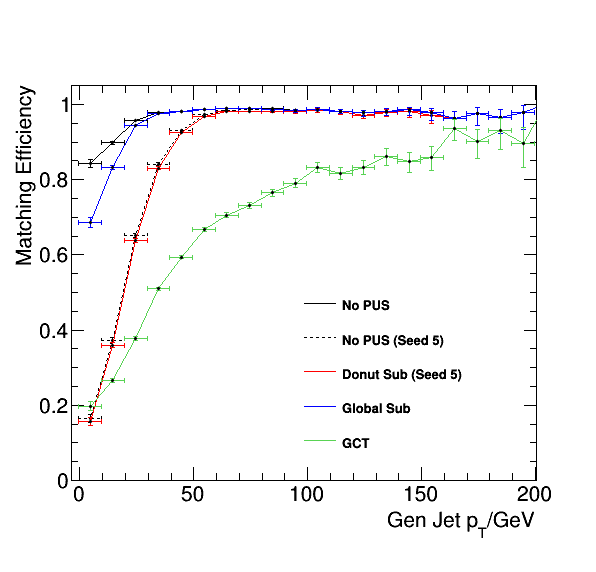
\includegraphics[width=7cm]{Figures/jet4}}
\hfill
\caption{Resolution before and after calibration. In \ref{fig:label:jet4} a comparison with the GCT is shown.}
\label{match}
\end{figure}
\section{PUS Testing}
\subsection{Reso}
In this section plots are shown for the highest $|\eta|$ bin as the detector perofrmance is expected to worsen with larger $|\eta|$ and so PUS will have the largest effect. The first test of any PUS scheme is the effect on the resolution. In an ideal post PUS scenario this will be flat as a function of NVTX. In figure \ref{fig:label:resolution1} this is plotted for a particular $p^{gen}_T$ and $\eta$ bin. It can be seen that the response flattens for both PUS regimes. This is summarised in \ref{fig:label:resolution2} where the gradient from the fit to the resolution plot is shown to reduce after PUS for a range of $p^{gen}_T bins$.  
\begin{figure}
\hfill
\subfigure[All jets\label{fig:label:resolution1}]{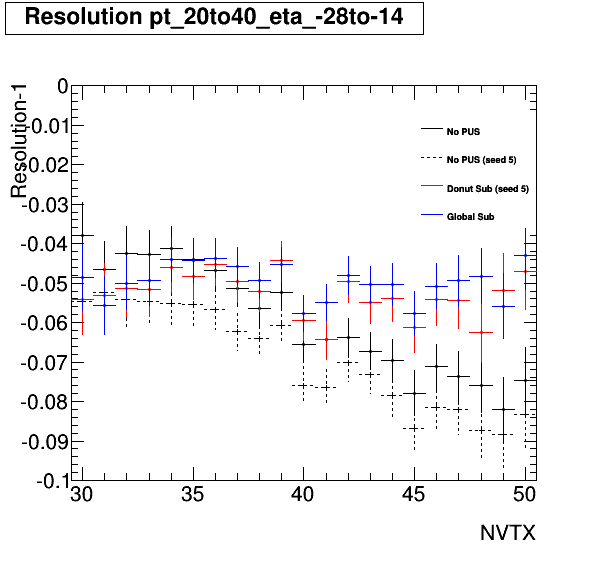
\includegraphics[width=7cm]{Figures/pt_20to40_eta_-28to-14}}
\hfill
\subfigure[All jets\label{fig:label:resolution2}]{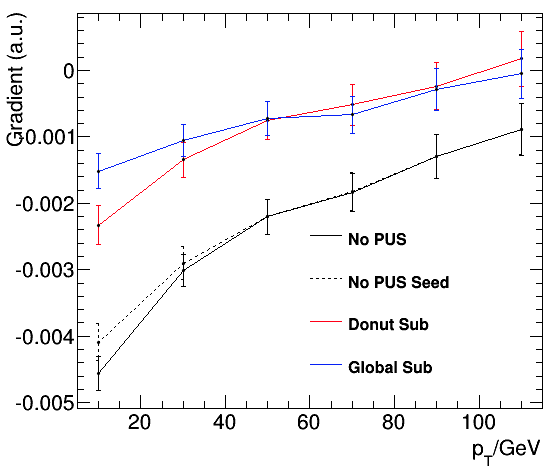
\includegraphics[width=7cm]{Figures/p1eta_14to28_calib_fits}}
\caption{In \ref{fig:label:resolution1} response versus NVTX is shown for a particular eta bin showing the response flattens after PUS. In \ref{fig:label:resolution2} the fit gradient for the response against NVTX for different $p_{T}$ bins is shown.}
\label{fig:label:resolution}
\end{figure}
\subsection{Rates}
The rate/efficiency is defined as the proportion of jets for signal/background passing a particular $p_{T}$ cut. For the trigger the key test is to see that the efficiency for signal may be maintained while reducing the background rate. Neutrino gun (PU40, 50ns) and ttbar (PU40, 50ns) samples were used as background and signal. In figure \ref{} the rate versus efficiency is plotted for the 4th jet. This shows PUS reducing the rate while maintaining efficiency. Performance compared to the GCT is shown to be greatly improved. This information is combined with the dependence on NVTX is shown in figure *. After PUS the rates are lower and the dependence on NVTX is reduced. 
\begin{figure}
\centering
    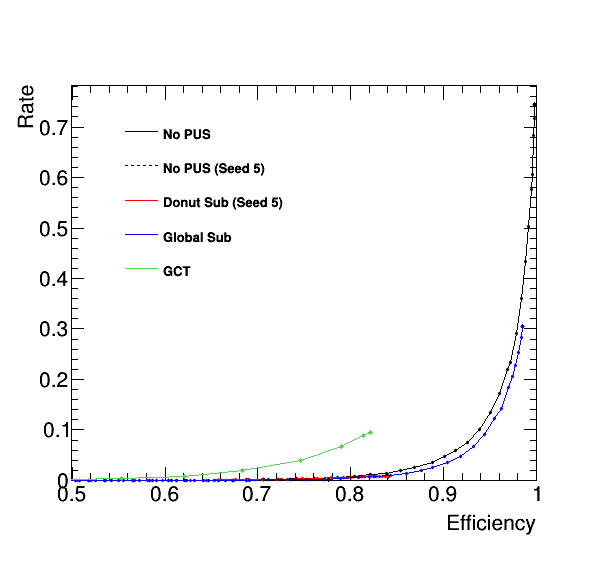
\includegraphics[width=0.8\textwidth]{Figures/rateeffjet4}
  \caption{Rate of a background (neutrino) sample against efficiency from a ttbar sample showing improvement after PUS.}
  \label{rateff}
\end{figure}
\begin{figure}
\hfill
\subfigure[All jets\label{fig:label:rateeff}]{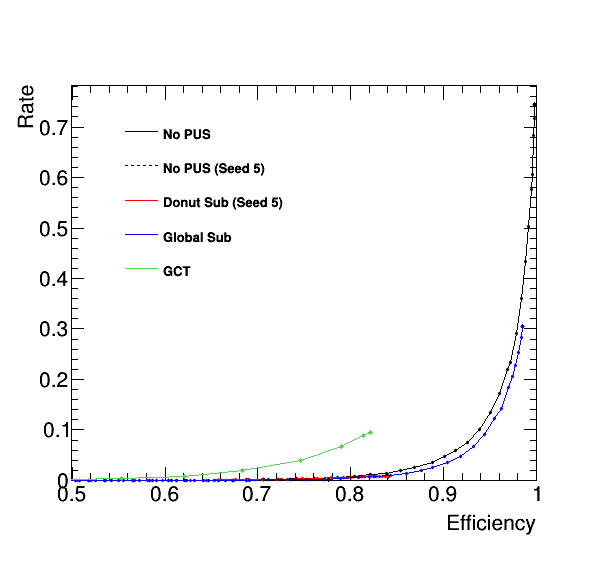
\includegraphics[width=7cm]{Figures/rateeffjet4}}
\hfill
\subfigure[All jets\label{fig:label:ratenvtx}]{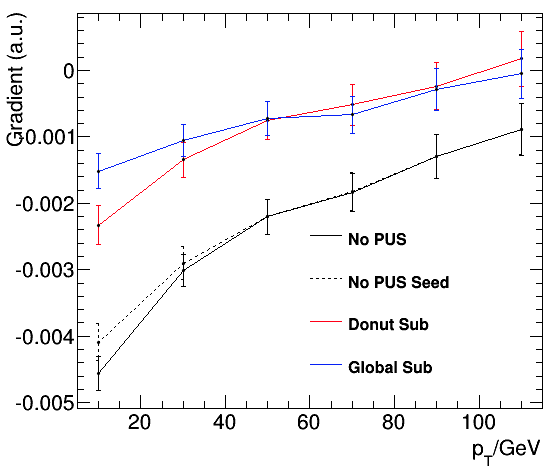
\includegraphics[width=7cm]{Figures/p1eta_14to28_calib_fits}}
\caption{In \ref{fig:label:resolution1} response versus NVTX is shown for a particular eta bin showing the response flattens after PUS. In \ref{fig:label:resolution2} the fit gradient for the response against NVTX for different $p_{T}$ bins is shown.}
\label{fig:label:resolution}
\end{figure}

